\section{Parser}
\textbf{Kontextfreie Sprache}
\begin{itemize}
    \item Kümmert sich um die syntaktische Analyse
    \item Input: Tokens (Terminalsymbole)
    \item Output: Syntaxbaum / Parse Tree
\end{itemize}
\subsection{Aufgabe}
\begin{itemize}
    \item Finde eindeutige Ableitung der Syntaxregeln, um einen gegebenen Input herzuleiten
    \item Analysiert die gesamte Syntaxdefinition (mit rekursiven Regeln)
    \item Erkennt, ob Eingabetext Syntax erfüllt
    \item Erzeugt Syntaxbaum
\end{itemize}
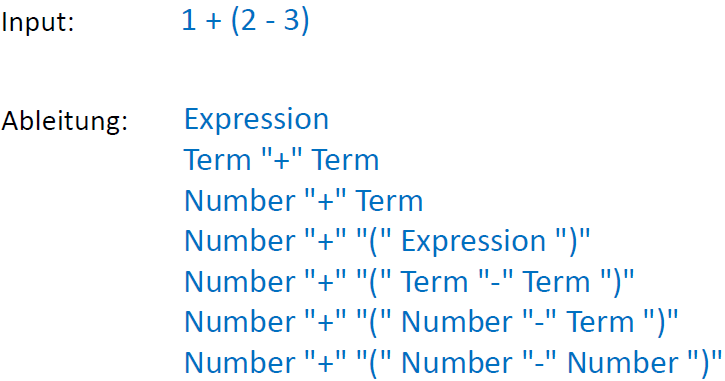
\includegraphics[width=0.5\linewidth]{/parser_aufgabe.png} 

\subsection{Parse Tree}
\begin{itemize}
    \item Concrete Syntax Tree
    \item Ableitung der Syntaxregeln als Baum wiedergespiegelt
    \item Kann generiert werden
\end{itemize}
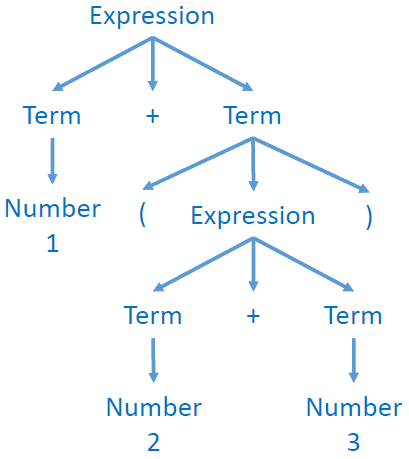
\includegraphics[width=0.3\linewidth]{/parse_tree.png} 

\subsubsection{Abstract Syntax Tree}
\begin{itemize}
    \item Unwichtige Details auslassen
    \item Struktur vereinfacht
    \item Für Weiterverarbeitung massgeschneidert
    \item Eigendesign nach Gusto des Compiler-Entwicklers
    \item Nur mit Selbstimplementation möglich
\end{itemize}
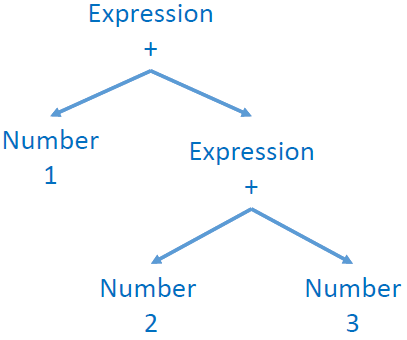
\includegraphics[width=0.3\linewidth]{/abstract_parse_tree.png} 

\subsection{Parser Strategien}
\subsubsection{Top-Down}
\begin{itemize}
    \item Beginne mit Start-Symbol
    \item Wende Produktionen an
    \item Expandiere Start-Symbol auf Eingabetext
    \item $Expr -> Term + Term -> ... -> 1 + (2 - 3)$
\end{itemize}
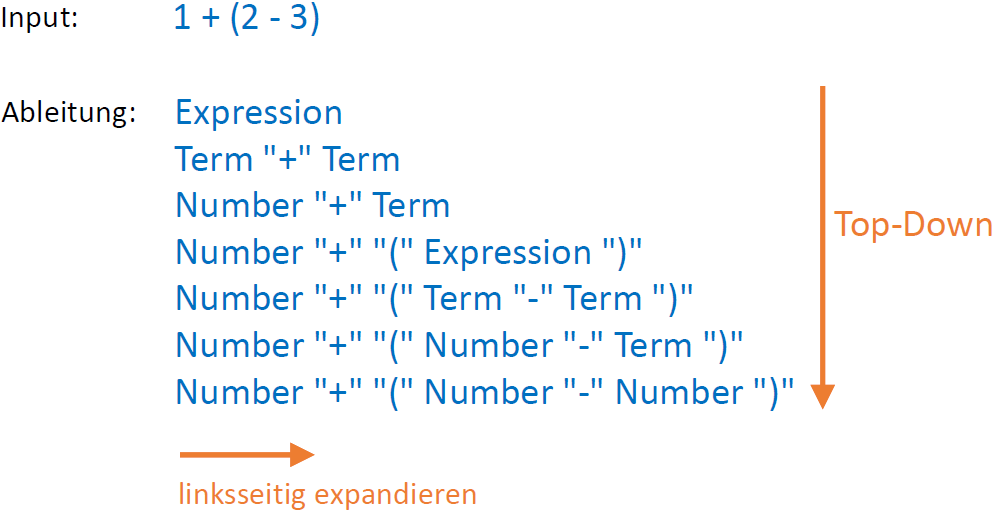
\includegraphics[width=0.5\linewidth]{/top_down.png} 

\subsubsection{Bottom-Up}
\begin{itemize}
    \item Beginne mit Eingabetext
    \item Wende Produktionen an
    \item Reduziere Eingabetext auf Start-Symbol
    \item $Expr <- Term + Term <- ... <- 1 + (2 - 3)$
\end{itemize}
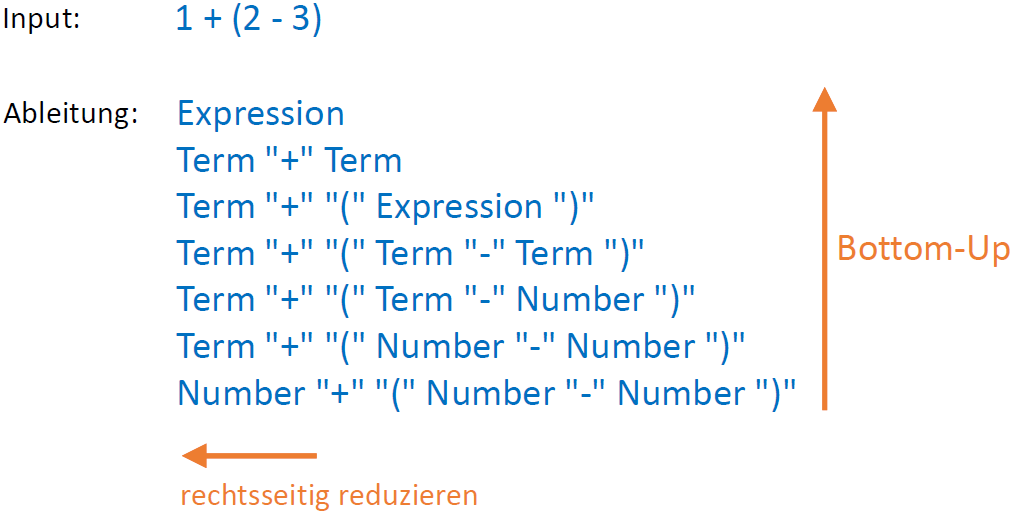
\includegraphics[width=0.5\linewidth]{/bottom_up.png} 

\subsection{Recursive Descent}
\begin{itemize}
    \item Pro Nicht-Terminalsymbol eine Methode
    \begin{itemize}
        \item Implementiert die Erkennung gemäss EBNF-Produktion
    \end{itemize}
    \item Vorkommen eines Nicht-Terminalsymbols in Syntax
    \begin{itemize}
        \item Aufruf der entsprechenden Methode
    \end{itemize}
    \item Funktioniert bei rekursiven und nicht-rekursiven Produktionen
\end{itemize}
\begin{lstlisting}
void parseExpression() {
    parseTerm();
    // ...
}
void parseTerm() {
    parseExpression();
    // ...
}
\end{lstlisting}

\subsection{Parser Gerüst}
\begin{lstlisting}
public class Parser {
    private final Iterator<Token> tokenStream;
    private Token current; // One Token Lookahead

    private Parser(Iterable<Token> tokenStream) {
        this.tokenStream = tokenStream.iterator();
    }

    public static ProgramNode parse(Iterable<Token> stream) {
        return new Parser(stream).parseProgram(); // Aufbasierte Klasse
    }
}
\end{lstlisting}

\subsubsection{Parser-Einstieg}
$Program = Expression$
\begin{lstlisting}
private ProgramNode parseProgram() {
    var classes = new ArrayList<ClassNode>();
    parseExpression();
    while (!isEnd()) {
        next();
        classes.add(parseClass());
    }
    return new ProgramNode(classes);
}
\end{lstlisting}

\subsubsection{Expression}
$Expression = Term { ( \dq +\dq | \dq -\dq ) Term }$
\begin{lstlisting}
Expression parseExpression() {
    var left = parseTerm();
    while(is(Tag.PLUS) || is(Tag.MINUS)) {
        var op = is(Tag.PLUS) ? Operator.PLUS : Operator.MINUS;
        next();
        var right = parseTerm();
        var left = new BinaryExpression(op, left, right);
    }
    return left;
}
\end{lstlisting}

\subsubsection{Term}
$Term = Number | \dq (\dq Expression \dq )\dq$
\begin{lstlisting}
Expression parseTerm() {
    if(isInteger()) {
        int value = readInteger();
        next();
        return new IntegerLiteral(value);
    } else if (is(Tag.OPEN_PARENTHESIS)) {
        next();
        var expression = parseExpression();
        if(is(Tag.CLOSE_PARENTHESIS)) {
            next();
        } else {
            error(); // missing closed parenthesis
        }
        return expression();
    } else {
        error(); // missing open parenthesis
    }
}
\end{lstlisting}

\subsection{One Symbol Lookahead}
\textbf{Statement}\\
$Assignment | IfStatement$
\begin{itemize}
    \item Bestimme mögliche Terminalsymbole, die mit einer Produktion ableitbar sind (FIRST-Menge)
    \item Benutze FIRST zur Entscheidung der Alternative beim zielorientierten Parsen
\end{itemize}
\begin{lstlisting}
void parseStatement() {
    if(isIdentifier()) { // FIRST(Assignment)
        parseAssignment();
    } else if(is(Tag.IF)) { // FIRST(IfStatement)
        parseIfStatement();
    } else {
        error();
    }
}
\end{lstlisting}

\subsection{Technische Syntax-Umformung}
\begin{itemize}
    \item Falls 1 Lookahead nicht reicht
\end{itemize}
\begin{lstlisting}
Statement = Assignment | Invocation
Assignment = Identifier "=" Expression
Invocation = Identifier "(" ")"
\end{lstlisting}

\begin{center}
    $\downarrow$
\end{center}

\begin{lstlisting}
Statement = Identifier (AssignmentRest | InvocationRest)
AssignmentRest = "=" Expression 
InvocationRest = "(" ")"
// Lookahead 1 reicht wieder
\end{lstlisting}

\subsubsection{Code Beispiel}
\begin{lstlisting}
var parseStatement() {
    var identifier = readIdentifier();
    next();
    if (is(Tag.ASSIGN)) {
        parseAssignmentRest(identifier);
    } else if (is(Tag.OPEN_PARENTHESIS)) {
        parseInvocationRest(identifier);
    } else {
        error();
    }
}
\end{lstlisting}